\section{Environmental Impact Assessment}

Environmental performance is a key consideration in the design of pharmaceutical manufacturing processes, particularly for solvent-intensive peptide synthesis routes such as semaglutide production. The SlimPepty facility has therefore been evaluated with respect to regulatory compliance and overall process sustainability. Chemical selection is also considered in the context of REACH regulations and the increasing regulatory scrutiny of solvents such as DMF. This section outlines the relevant environmental legislation, key process modifications to reduce the environmental footprint of the plant, and quantitative estimates of emissions and waste streams.

To minimise environmental impact, several measures have been incorporated into the process design. These include transitioning from a fully SPPS route to a hybrid SPPS/liquid-phase peptide synthesis (LPPS) approach to reduce solvent consumption, evaluating alternative solvents to reduce toxicity, and implementing dedicated wastewater and waste treatment systems to reduce overall waste generation and improve process sustainability.

\subsection{Local Legislation: Environment}

For the purposes of this report, the proposed SlimPepty facility is assessed against the EU/UK environmental framework. For a semaglutide process based on solvent-intensive peptide synthesis and reverse-phase high-performance liquid chromatography (RP-HPLC) purification, the main environmental concerns are solvent-rich liquid waste, aqueous effluent, volatile organic compound (VOC) emissions, and hazardous solid wastes such as spent SPPS resin and contaminated treatment residues.

\subsubsection{Industrial Emissions and Environmental Permitting}

Under the EU framework, API manufacture is controlled through integrated pollution prevention under the Industrial Emissions Directive (IED) \cite{EU_IED_2010}, with emissions to air, water and land managed through permit conditions based on Best Available Techniques or BAT. In the UK, an equivalent approach is implemented through the Environmental Permitting (England and Wales) Regulations 2016 \cite{UK_EPR_2016}. Accordingly, the plant design should assume that environmental monitoring, documented operating procedures, and appropriate emission-control systems form part of normal regulatory compliance rather than optional measures.

\subsubsection{Wastewater and Liquid Effluent}

The semaglutide process generates aqueous and solvent-containing streams from washing, purification and cleaning operations, so wastewater must be segregated and treated prior to discharge. EU expectations for chemical-sector wastewater management are set out in the BAT conclusions for common wastewater and waste gas treatment systems \cite{EC_BAT_2016}, while protection of receiving waters is established more broadly under the Water Framework Directive \cite{EU_WFD_2000}. These requirements support source segregation, equalisation, neutralisation, solvent recovery where feasible, and suitable end-of-pipe treatment before discharge.

\subsubsection{Air Emissions and Solvent Management}

The main atmospheric concern for this plant is VOC release from the handling of organic solvents, particularly DMF in peptide synthesis and acetonitrile in purification. For organic fine chemical manufacture, the relevant BAT guidance recommends closed solvent handling, condensers, vapour recovery and abatement of residual off-gases \cite{EC_OFC_BREF_2006}. This supports the wider design objective of reducing solvent consumption and minimising fugitive solvent losses to the environment.

\subsubsection{Solid and Hazardous Waste Disposal}

Spent SPPS resin, contaminated filtration solids, off-spec product and residues from effluent treatment should be managed as hazardous waste. Under the EU waste framework \cite{EU_WasteDir_2008}, such wastes must be classified, segregated and transferred through controlled disposal routes with full documentation and traceability, while prevention, reuse and recovery remain preferable wherever technically feasible.

\subsubsection{Chemical Regulation and Solvent Selection}

Chemical selection is also relevant from an environmental compliance perspective. The general framework for managing substances of concern is provided by REACH \cite{EU_REACH_2006}, while DMF is subject to a specific restriction under Annex XVII \cite{EU_REACH_DMF_2021}. Therefore, any reduction in DMF usage or substitution with a less problematic solvent would improve the long-term environmental robustness of the process.

\subsection{Solvent Usage and Choices}
\label{sec:solvent_usage_choices}

One of the primary objectives of this project is to reduce solvent usage by 50\%. As discussed earlier, the process mass intensity (PMI) for semaglutide manufacturing is approximately 14,000~L of solvent per kg of semaglutide, which was taken as the baseline. Accordingly, the target is to reduce solvent consumption to 7,000~L of solvent per kg of semaglutide.

To achieve this, the first major process modification involved transitioning from a traditional SPPS route to a hybrid SPPS/LPPS approach. LPPS is known to require significantly lower solvent volumes and enables the use of less toxic solvents compared to conventional SPPS. Additionally, solvent recycling from the effluent streams was also considered; but the recovered solvent needs to have a high purity in order to be recycled back into the process. Following the implementation of these process modifications, the PMI was reduced to approximately 3460~L of solvent per kg of semaglutide, representing a reduction greater than the initial target and indicating a significant improvement in the overall sustainability of the process.

Furthermore, DMF accounts for approximately 40\% of the organic solvents used in SPPS, primarily because very large volumes are consumed during the repeated washing cycles required between each coupling and deprotection step, in addition to DMF's roles in swelling resin beads and dissolving protected amino acids and coupling reagents. While our manufacturing site is in the United States, it is still relevant that DMF is classified as a Substance of Very High Concern (SVHC) in the EU and the UK \cite{ECHA_SVHC} and is subject to increasingly stringent regulatory controls, reflecting the broader direction of travel for solvent selection in pharmaceutical manufacturing. So, replacing DMF would materially reduce the toxicity profile of the solvent system and could lower the overall solvent impact associated with high-volume SPPS washing, which led to the consideration of alternative solvents.

When evaluating alternative solvents for the process, several key requirements must be considered. These include the chemical compatibility of the solvent with the reactants and intermediates, its influence on reaction kinetics, and its overall compatibility with the process conditions. In addition, theoretical feasibility must be established to ensure that candidate solvents can effectively substitute the currently used solvent, DMF, without negatively impacting reaction performance or product quality. Based on these criteria, N-butylpyrrolidinone (NBP) \cite{Kumar_NBP_2020} seemed like the best fit for comparison against DMF. Based on the analysis in Section~\ref{sec:solvent_usage_choices}, DMF was chosen as the final solvent.

\subsection{Waste Disposal}
\label{sec:waste_disposal}

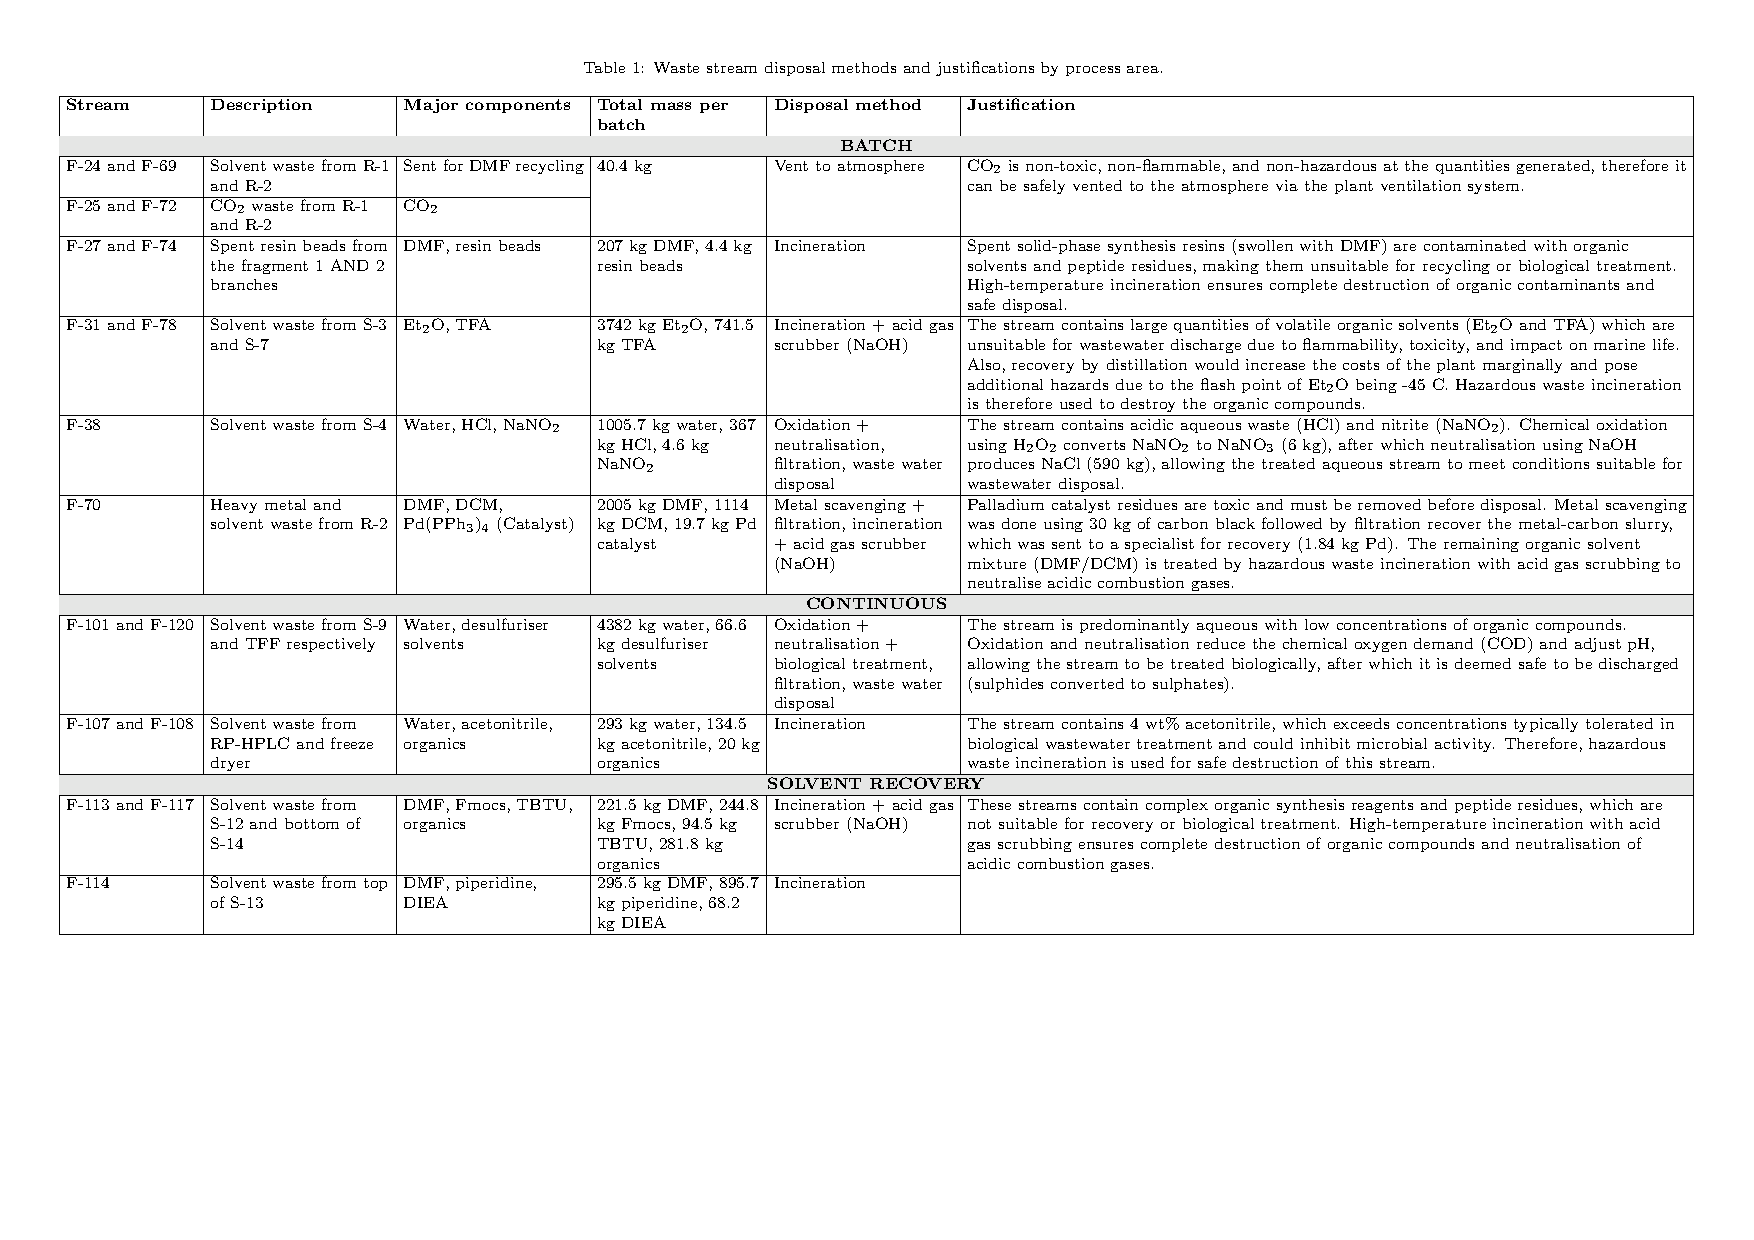
\includepdf[pages=-,landscape=true]{figures/tables/waste_stream_disposal_table.pdf}

Table~\ref{tab:emissions_effluents} summarises the main emissions and effluents generated from waste treatment and incineration, together with batch and annual quantities.

Appendix~\ref{app:incineration} shows the total mass of compounds sent for incineration as well as the corresponding NaOH requirement for flue gas scrubbing. Table~\ref{tab:emissions_effluents} shows the main emissions and effluents generated from the waste treatment and incineration processes, including their quantities.

\begin{table}[htbp]
    \centering
    \caption{Main emissions and effluents from waste treatment and incineration.}
    \label{tab:emissions_effluents}
    \small
    \begin{tabularx}{\textwidth}{|>{\raggedright\arraybackslash}X|c|c|>{\raggedright\arraybackslash}X|}
        \hline
        \textbf{Emissions/effluents} & \textbf{kg/batch} & \textbf{tons/year} & \textbf{Limits} \\
        \hline
        CO$_2$                       & 19600             & 1019.2             &                 \\
        \hline
        H$_2$O                       & 9220              & 479.44             &                 \\
        \hline
        NO$_x$                       & trace             & -                  &                 \\
        \hline
        HCl (removed in scrubber)    & 957               & 49.764             &                 \\
        \hline
        HF (removed in scrubber)     & 390               & 20.28              &                 \\
        \hline
        SO$_2$ (removed in scrubber) & 50                & 2.6                &                 \\
        \hline
        Waste water                  & 6250              & 325                &                 \\
        \hline
    \end{tabularx}
    \normalsize
\end{table}

Appendix~\ref{app:waste_treatment} summarises the chemicals and equipment required for the waste treatment plant, including chemical consumption per batch, equipment specifications, capital costs, and energy requirements. These data were used to estimate the annual cost of the waste treatment system, which was calculated to be \$342,085. The total waste generated by the process is approximately 19,240~kg per year, corresponding to a treatment cost of about \$0.34 per kg of waste.

It is to be noted that this estimate only includes capital costs for treatment equipment (e.g., incinerator, scrubber, oxidation and neutralisation tanks, filtration units, metal scavenging and biological treatment tanks) and operating costs for chemicals such as NaOH, carbon black, H\textsubscript{2}O\textsubscript{2}, biomass, and electricity. It does not include additional industrial costs such as labour, equipment maintenance, sludge disposal, emissions monitoring, regulatory compliance, or waste transport, which can significantly increase overall treatment costs in pharmaceutical facilities.

\subsection{Utilities}
\label{sec:utilities}

A detailed evaluation of the utilities required for plant operation is presented in this subsection. Excluding waste treatment, the total installed electrical load of the plant is 111.8~kW, corresponding to the combined power requirements of pumps and mixers. The plant also requires approximately 1~gpm of industrial water, equivalent to approximately 2000~m$^3$/year, which is subsequently purified using reverse osmosis and electrodeionisation for use in pharmaceutical processing. Additional utilities required to support process operation and temperature control include chilled water, propylene glycol-water brine refrigeration, and low- and medium-pressure steam, as described in this subsection.

From a sustainability perspective, the process incorporates solvent recovery and on-site waste treatment systems to reduce solvent consumption and minimise environmental emissions. In addition, propylene glycol-water brine was selected as the refrigeration medium rather than ethylene glycol due to its lower toxicity and favourable safety profile for pharmaceutical manufacturing.

\subsection{Greenhouse Gas Emissions}
\label{sec:ghg_emissions}

Carbon dioxide emissions from the plant include both direct (Scope~1) and indirect (Scope~2) sources. Annual Scope~1 CO$_2$ emissions are approximately 1,020~ton/year, primarily originating from process vents and incineration flue gases. Indirect CO$_2$ emissions (Scope~2) are estimated at approximately 600~ton/year, arising from the electricity demand of the main process and waste treatment operations, as well as the steam requirements of the plant. SO$_2$ and trace quantities of NO$_x$ are also produced during the incineration process, but these emissions are subsequently treated in a caustic scrubber, ensuring that they are not directly released to the environment. These values provide an overall estimate of the greenhouse gas emissions associated with the facility's operation. A summary of related emissions and treatment calculations is provided in Appendix~\ref{app:incineration} and Appendix~\ref{app:waste_treatment}.

The estimated emissions were compared with regulatory limits specified under the IED and the BAT conclusions for waste incineration and chemical sector emissions. Acid gases generated during incineration, including SO$_2$, HCl and HF, are removed through a caustic scrubbing system prior to atmospheric release. The predicted emission levels therefore remain below typical BAT-associated emission levels for these gases, demonstrating compliance with applicable environmental regulations.

Potential reductions in greenhouse gas emissions could be achieved through both operational and energy-sourcing strategies. Scope~1 emissions could be reduced by improving energy efficiency, recovering heat from incineration flue gases, or minimising the amount of waste sent for incineration through more efficient solvent recovery and waste reduction measures. Scope~2 emissions could be reduced by sourcing electricity from a lower-carbon energy mix than the current grid mix in North Carolina. This could include the use of renewable electricity through power purchase agreements or on-site renewable generation such as solar power. Increasing the proportion of renewable energy used to meet the plant's electricity demand would significantly reduce the indirect carbon footprint associated with process operation.
